\documentclass[utf8]{FrontiersinHarvard} % for articles in journals using the Harvard Referencing Style (Author-Date), for Frontiers Reference Styles by Journal: https://zendesk.frontiersin.org/hc/en-us/articles/360017860337-Frontiers-Reference-Styles-by-Journal
%\documentclass[utf8]{FrontiersinVancouver} % for articles in journals using the Vancouver Reference Style (Numbered), for Frontiers Reference Styles by Journal: https://zendesk.frontiersin.org/hc/en-us/articles/360017860337-Frontiers-Reference-Styles-by-Journal
%\documentclass[utf8]{frontiersinFPHY_FAMS} % Vancouver Reference Style (Numbered) for articles in the journals "Frontiers in Physics" and "Frontiers in Applied Mathematics and Statistics" 

%\setcitestyle{square} % for articles in the journals "Frontiers in Physics" and "Frontiers in Applied Mathematics and Statistics" 
\usepackage{url,hyperref,lineno,microtype,subcaption}
\usepackage[onehalfspacing]{setspace}

\linenumbers
% \documentclass[draft]{agujournal2019}
% \usepackage{url}
% \usepackage{lineno}
% \usepackage{soul}
\usepackage{minted}

\def\keyFont{\fontsize{8}{11}\helveticabold }
\def\firstAuthorLast{Shumko {et~al.}}
\def\Authors{M. Shumko\,$^{1,2,*}$, B. Gallardo-Lacourt\,$^{1,3}$, E. Donovan\,$^{4}$, D. Chaddock\,$^{4}$, E.L. Spanswick\,$^{4}$, A.J. Halford\,$^{1}$, I. Thompson, and K.R. Murphy}

\def\Address{
    $^{1}$NASA's Goddard Space Flight Center, Greenbelt, Maryland, USA \\
    $^{2}$Department of Astronomy, University of Maryland, College Park, Maryland, USA\\
    $^{3}$Department of Physics, The Catholic University of America, Washington, DC, USA\\
    $^{4}$University of Calgary in Calgary, Alberta, Canada
}
\def\corrAuthor{M. Shumko}

\def\corrEmail{msshumko@gmail.com}

\begin{document}
\onecolumn
\firstpage{1}

\title[AuroraX, PyAuroraX, and aurora-asi-lib]{AuroraX, PyAuroraX, and aurora-asi-lib: a user-friendly auroral all-sky imager analysis framework} 

\author[\firstAuthorLast ]{\Authors} %This field will be automatically populated
\address{} %This field will be automatically populated
\correspondance{} %This field will be automatically populated

\extraAuth{}


\maketitle


\begin{abstract}
\section{}
Within the context of the Heliophysics Observatory, ground-based data is emerging as core to understanding multi-scale coupling in the “system of systems” era. Historically, the patchwork of ground-based instrumentation has required customized solutions for assessing data relevance, accessing data, and then ultimately using each individual network alongside other assets. We present here a new approach for data discovery and utilization for one such ground-based instrument, the all-sky imager (ASI). AuroraX aims to enable efficient and seamless data discovery and utilization for the world's ground-based auroral imagers. The core of AuroraX's science data interface is three main tools: the AuroraX website (\url{https://aurorax.space/}); PyAuroraX, an application program interface to the AuroraX website written in Python; and aurora-asi-lib, an auroral ASI library also written in Python. Together, these three tools enable a rapid and painless end-to-end analysis of the aurora. One such example is a conjunction study: AuroraX---or the PyAuroraX---can be used to quickly identify conjunctions between numerous ground- and space-based instruments and quickly look at keograms from the available imagers to look for the aurora. The list of conjunctions, together with aurora-asi-lib, can be then used to download, load, and analyze ASI data directly on a personal computer.
\tiny
 \keyFont{ \section{Keywords:} THEMIS, REGO, aurora, all-sky-imager, precipitation, python}
\end{abstract}

\section{Introduction}\label{intro}
Since the 1960s the space physics community has utilized optical ground-based instrumentation that has led to discoveries from which great advancements in the field have been derided. Some of these discoveries include the early description of a substorm introduced by \citet{Akasofu1964}, and several descriptions of new phenomena that highlight the tight connections between the magnetosphere and ionosphere \cite[e.g.][]{Angelopoulos2008, Jones2013, Shumko2021}. These discoveries were possible with a multitude of instruments. 

Meridian Scanning photometers (MSP), such as the Canadian Auroral Network for the OPEN (Origins of Plasmas in Earth's Neighborhood) Program Unified Study (CANOPUS) array, were first utilized for remote sensing the high-latitude ionosphere \citep[e.g.][]{Rostoker1995}. These one-dimensional MSPs were later followed by two-dimensional All-sky Imagers (ASIs) that took the space physics field into a deeper understanding of the ionosphere-magnetosphere coupled system. In the present day, the space physics community has carried a long legacy of ground-based optical instruments, including the large array from the Time History of Events and Macroscale Interactions during Substorms (THEMIS) ASI observatories \citep{Donovan2006, Mende2009}. Currently, many different optical arrays are in operation or are in development including THEMIS, REGO, MANGO, TREx, and PWING  \citep[e.g.][]{Liang2016, Shiokawa2017, Lyons2019, Gillies2019}. These modern ASIs work continuously in high temporal and spatial resolution: each camera producing thousands of images per night.

The rapidly increasing volume of imager data, together with unique data formats, significantly burdens space physicists with mundane and duplicated software engineering tasks---download data, load and correctly parse the data, etc. This unnecessary burden can also lead to mistakes in analysis software that may require unnecessary troubleshooting time from the ASI team, or more worrisome---lead to inaccurate and misleading findings getting published. Thus, robust auroral analysis tools are required.

We introduce the AuroraX project that aims to overcome the above issues by providing three robust tools that most auroral researchers need. The first tool is the AuroraX website (https://aurorax.space/) that can quickly plot keograms, show what imagers operated at a given time, and calculate conjunctions between numerous ground- and space based instruments. The second tool is the PyAuroraX, a Python library that interfaces with the AuroraX website to automate the use of the its services from a personal computer. The third tool is aurora-asi-lib, a Python all-sky imager library that provides functions to download, load, analyze, and visualize THEMIS and REGO ASI data. 

\section{AuroraX}\label{aurorax}

\subsection{The AuroraX Website}
The AuroraX website, located at (\url{https://aurorax.space/}) is designed to be the first place to start your auroral analysis. The primary objective of AuroraX is to enable data mining and analysis of existing and future auroral data, enabling key science and enhancing the benefits of the world's investment in auroral instrumentation. This is being accomplished with the development of key systems/standards for uniform metadata generation and search, image content analysis, interfaces to leading international tools, and a community involvement that includes more than 80\% of the world's data providers. The AuroraX website contains three browser applications: the Swarm-Aurora Keogram Browser, a Conjunction Search Engine, and the virtual observatory. \textcolor{blue}{What is the difference between Swarm-Aurora and AuroraX? Is Swarm-Aurora the legacy website? It is confusing to me as is.} 

The primary goal of the Keogram Browser is to provide an easy and scientifically productive tool for viewing summary data from ground-based auroral imaging instruments. AuroraX makes keograms given the date and one or more ASI arrays (sets of imagers). A keogram is a compression of sequential ASI images into a single image that shows pixel intensity as a function of latitude and time. Typically, they are assembled by looping over every image and copying pixels that are oriented North-South through zenith (or through a custom path such a path of a satellite). Objects in the sky such as auroral arcs, pulsating aurora, substorms, clouds, the moon, etc. all have unique keogram signatures that allow for a quick classification. Figure \ref{fig1}(A) shows the THEMIS ASI keograms from the available imagers on 9 March 2008; It shows a sequence of substorms that were simultaneously observed by many THEMIS ASIs. 

\begin{figure}
    \centering
    \includegraphics[width=0.9\textwidth]{figures/fig1.jpg}
    \caption{The \url{https://aurorax.space/} website. Panel (A) shows the daily keogram browser. Panel (B) shows the conjunction finder with keograms. And lastly, panel (C) shows the conjunctions in list form.}
    \label{fig1}
\end{figure}

The Conjunction Search Engine finds conjunctions between ground-based ASIs and space-based instruments. It helps researchers streamline the process of ``event discovery", quickly narrowing down the possible times that may contain interesting data. The web interface provides a  few ways to specify and search for conjunctions from the dropdown menu. The menus include the start and end time, maximum distance between instruments, conjunction type (such as geographic or magnetic footprints in either hemispheres using SSCWeb for space-based instruments, and using AACGM \citep{Shepherd2014} for ground-based instruments), ``criteria blocks" to specify what instruments to calculate the conjunctions of, and metadata filters to filter the results by weather and auroral conditions. Figure \ref{fig1}(B) shows a list of all conjunctions identified between the TREx ASIs and all space-based instruments that are cataloged within AuroraX. Clicking on one of the conjunctions leads to a detailed view that we show in Fig. \ref{fig1}(C). This view shows a map with the ASI fields of view and the Swarm orbits superposed. The keograms from the available ASIs are shown on the right hand side of the website. Thus, the conjunction search engine allows a researcher to quickly identify, filter, quantify good conjunctions.

The Virtual Observatory aims at providing interactive visualizations and data browsing tools to quickly navigate the vast amount of data available. These web-based applications are geared towards identifying auroral events of interest using summary data of different types. The Virtual Observatory currently has two web interfaces available: Keogramist, and the Event Explorer. Keogramist is designed with the goal of streamlining the ``event discovery" process by using ASI keograms and timelapse movies. The interface has the ability to filter different ASI arrays and sites, or filter on arbitrary metadata in the AuroraX database (ie. percentage of green channel content, image content derived from machine learning models, etc.). The Event Explorer is a 3D visualization of AuroraX ephemeris data with ground-based auroral images projected onto an interactive globe. This tool is designed to assist with visualizing auroral data and evaluating possible conjunctions using a more interactive and global interace. The auroral images are mapped to a 1024x512 grid covering $-180^\circ$ to $180^\circ$ degrees in longitude, and $-90^\circ$ to $90^\circ$ latitude ($0.33^\circ$ and $0.35^\circ$ longitude and latitude resolution), and visualized onto the globe. The grid format was first developed by NOAA and used as part of their 30-min auroral prediction OVATION model outputs. AuroraX has adopted this grid format and the API provides the ability to upload and retrieve grid files for various ground-based ASI arrays (ie. THEMIS, REGO, TREx). The Event Explorer also provides a visual representation of spacecraft geographic positions and magnetic footprints provided by the AuroraX API.

\subsection{PyAuroraX}
In addition to the web-based tools, AuroraX also provides users with the ability to interact with the platform using custom-written software. This is achieved using the AuroraX RESTful API and subsequent client libraries. PyAuroraX is the Python client library for AuroraX, and allows users to retrieve from or upload data to AuroraX.

PyAuroraX's core functionality allows for users to perform conjunction, ephemeris, and data product searches using Python code. For example, the \verb|pyaurorax.conjunctions.search()| function can be used to search AuroraX for conjunctions in the same way the AuroraX website allows (\url{https://aurorax.space/conjunctionSearch/standard}). The below Python code shows how to perform a simple search, asking AuroraX to find all conjunctions between several instruments from the THEMIS ASI array and any Swarm spacecraft.

\begin{minted}{python}
import pyaurorax
import datetime

# define search parameters
start = datetime.datetime(2019, 1, 1, 0, 0, 0)
end = datetime.datetime(2019, 1, 3, 23, 59, 59)
ground_params = [
    {
        "programs": ["themis-asi"],
        "platforms": ["fort smith", "gillam"],
    }
]
space_params = [
    {
        "programs": ["swarm"],
        "hemisphere": ["northern"],
    }
]
distance = 500

# perform conjunction search
s = pyaurorax.conjunctions.search(start=start,
                                  end=end,
                                  distance=distance,
                                  ground=ground_params,
                                  space=space_params,
                                  verbose=True)
\end{minted}

Another example of using PyAuroraX is to search the ephemeris data to retrieve all 1-min timestamps when a machine learning model predicted that Amorphous Pulsating Aurora (APA) was visible in the imager's field of view \cite{Grono2020}. This list of timestamps could then be used in further analysis with other in-situ or ground-based instrument data outside of AuroraX.

The AuroraX Documentation website provide more in-depth technical details about AuroraX, and provides a ``Developer Zone" with extensive examples of writing software in various supported languages (ie. Python, Javascript, IDL, etc.). This website is available at \url{https://docs.aurorax.space}.

\section{aurora-asi-lib}\label{aurora-asi-lib}
The final component of AuroraX is aurora-asi-lib, henceforth referred to (and imported) as asilib. It enables researchers to apply common data analysis tasks to the THEMIS and REGO ASI image data on a personal computer. Here we overview the main functions, while the online documentation has more examples, a tutorial, and a thorough API reference \url{https://aurora-asi-lib.readthedocs.io/}. \textcolor{red}{Merge these docs with \url{https://docs.aurorax.space/}?}

As we tour the asilib functions, keep in mind that asilib is designed to manage the lower-level tasks. For example, if you want to load the image data via \verb|asilib.load_image()|, asilib will attempt to download it if it is not already saved on your computer. Likewise, if you call \verb|asilib.plot_keogram()|, it will automatically load (and download if necessary) the ASI data before plotting it. For reference, Figs. 2-4 were made using the code in a Jupyter Notebook that is provided as supplemental material in both the ipynb and pdf formats.

\subsection{Download and load ASI image and skymap data}
Let us start with the four functions that download and load ASI image and skymap data: 

\begin{itemize}
      \item \verb|asilib.download_image()|,
      \item \verb|asilib.download_skymap()|,
      \item \verb|asilib.load_image()|, and
      \item \verb|asilib.load_skymap()|
\end{itemize} that are described below.

The \verb|asilib.download_image()| function downloads the level 1 hourly Common Data Format (CDF) files from \url{http://themis.ssl.berkeley.edu/data/themis/thg/l1/asi/} for THEMIS, and \url{http://themis.ssl.berkeley.edu/data/themis/thg/l1/reg/} for REGO. The files are saved in the \verb|asilib.config['ASI_DATA_DIR']| directory that is \verb|~/asilib-data/| by default, and is customizable.

The \verb|asilib.download_skymap()| function downloads all of the skymap files from \url{https://data.phys.ucalgary.ca/sort_by_project/THEMIS/asi/skymaps/} and \url{https://data.phys.ucalgary.ca/sort_by_project/GO-Canada/REGO/skymap/} for a given set of \verb|asi_array_code| and \verb|location_code|. The skymap files are in the Interactive Data Language (IDL) \verb|.sav| file format. Noteworthy is that \verb|asilib| downloads all of the skymap files for a given imager because the skymaps are only valid for a set time period (typically a year; see the logic for \verb|asilib.load_skymap()| that is described below). Lastly, asilib converts the longitudes from $[0^\circ, 360^\circ]$ to $[-180^\circ, 180^\circ]$.

As the name implies, \verb|asilib.load_image()| loads into memory and returns the ASI time stamps and images for a specified imager. This function can load both single and multiple images: a single time stamp and image if \verb|time| is provided, and multiple time stamps and images if \verb|time_range| is provided. As previously mentioned, \verb|asilib.load_image()| will try to download an hourly CDF file if it does not exist locally.

\verb|asilib.load_skymap()| is the last noteworthy input function; it loads the relevant skymap file into memory and returns the data in a dictionary. A relevant skymap file is the latest one before the specified \verb|time|. As with \verb|asilib.load_image()|, \verb|asilib.load_skymap()| will attempt to download the skymap files if they are not already downloaded.

Before we discuss the plotting functions, we emphasize that the \verb|asilib.download_image()| and \verb|asilib.download_skymap()| functions are often unnecessary to call since they are called by \verb|asilib.load_image()| and \verb|asilib.load_skymap()|. However, the download functions are very useful if you need to download ASI image and calibration data in bulk. For example, these calls are useful to analyze data offline.

\subsection{Plotting single images}

The \verb|asilib| provides two ways to plot a single ASI image:

\begin{itemize}
      \item \verb|asilib.plot_fisheye()| and
      \item \verb|asilib.plot_map()|.
\end{itemize}

One common way to visualize all-sky images is with \verb|asilib.plot_fisheye()|. It plots the raw ASI images oriented with North at the top and East to the right of each image. The term fisheye comes from the fisheye lens that expands the imager's field of view to nearly $180^\circ$. Figure \ref{fig2}a,c show an example of an auroral arc observed concurrently by the THEMIS and REGO ASIs stationed at Rankin Inlet (RANK). If you don't override the parameters, the color map is automatically chosen: black-to-white for THEMIS and black-to-red for REGO. The default color scale is dynamically calculated using percentile logic described in the documentation.

Another common way to visualize images is by projecting the fisheye image onto a geographic map using \verb|asilib.plot_map()|. asilib uses the skymap files to map each pixel's vertices to a (latitude, longitude) point at an aurora emission altitude (typically assumed 110 km for THEMIS and 230 km for REGO \cite{Donovan2006, Liang2016}). Figure \ref{fig2}b,d show the fisheye images mapped to 110 km altitude. By default, pixels that look at elevation $< 10^\circ$ are not mapped due to nearby obstructions and the stretching of pixels closest to the horizon. And lastly, \verb|asilib.plot_map()| provides default map styles that can be overwritten with a custom \verb|cartopy| \cite{Cartopy} map passed in via the \verb|ax| keyword argument.

\begin{figure}
      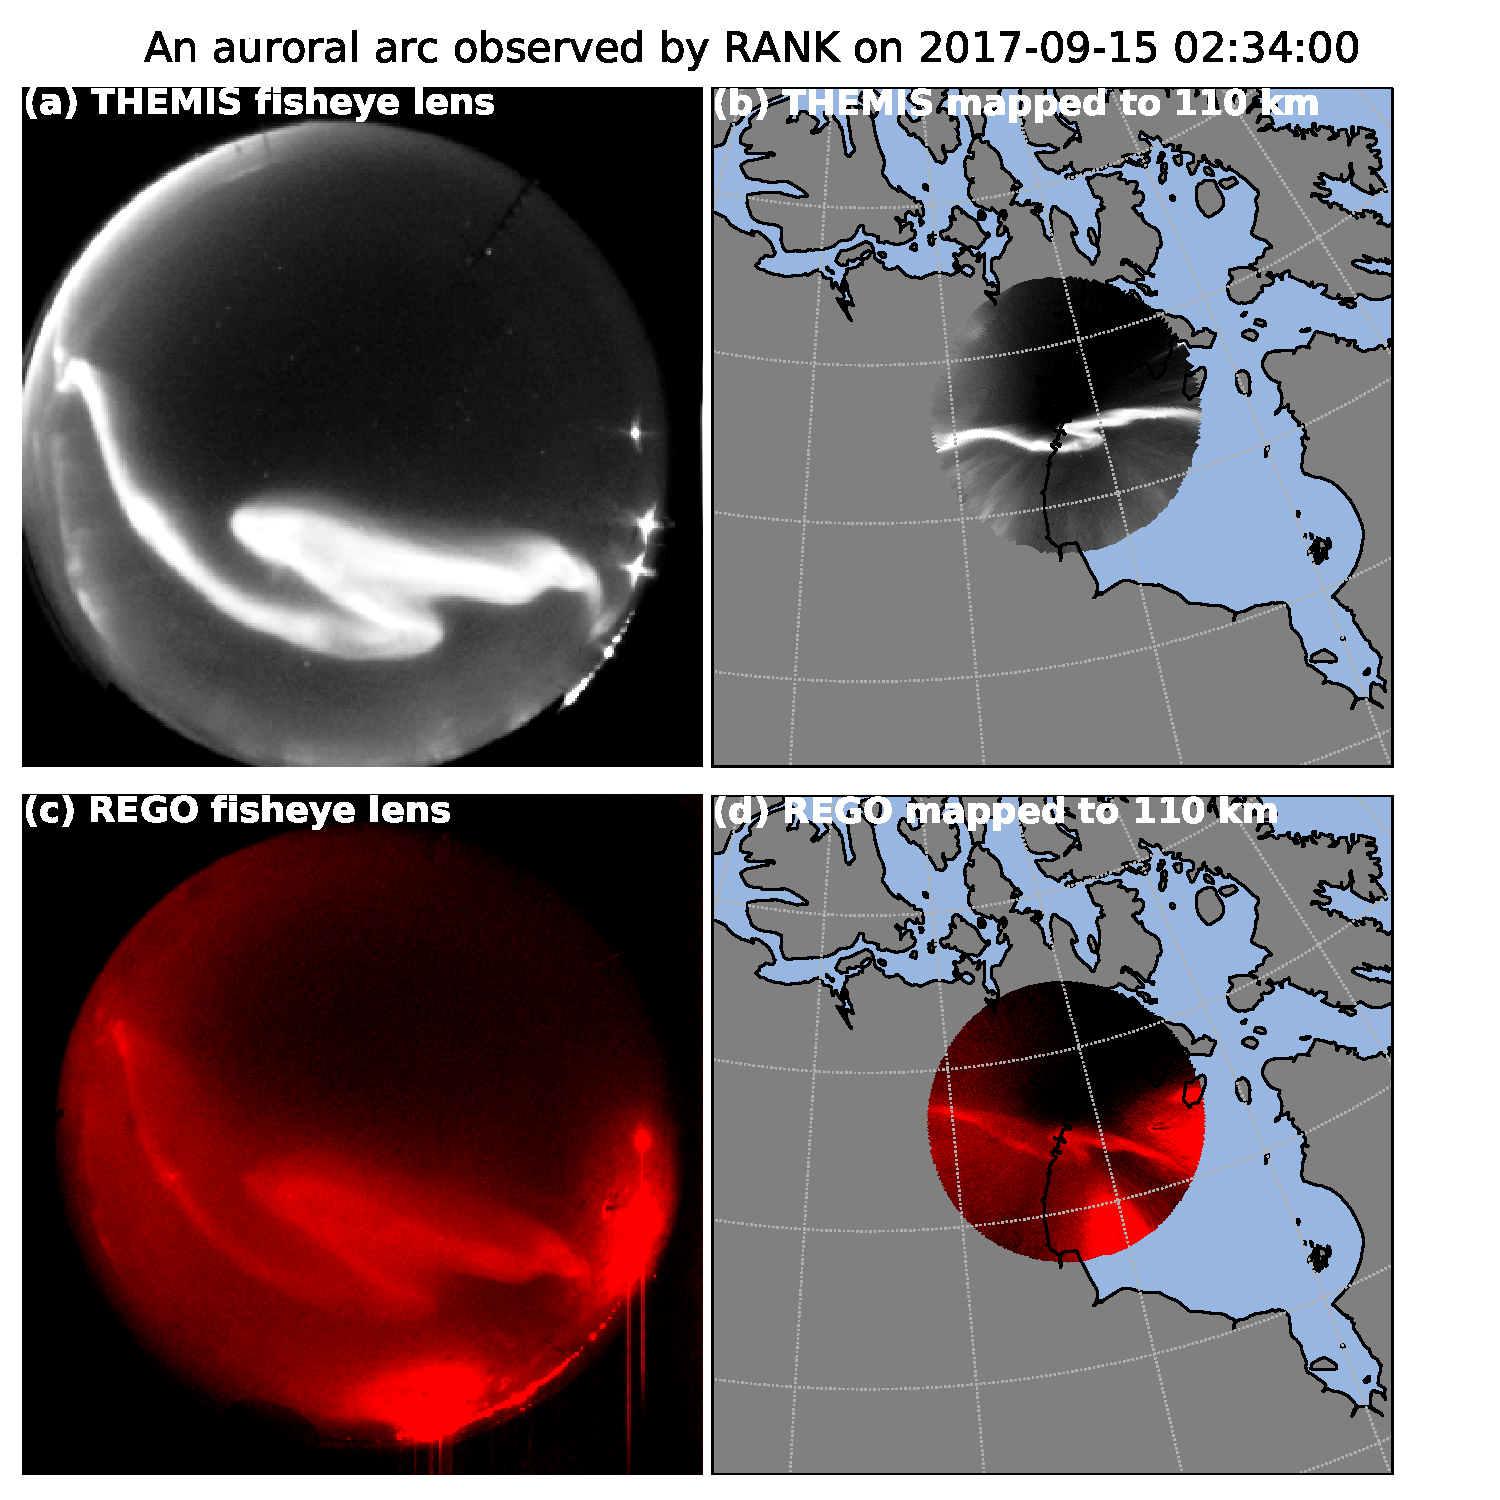
\includegraphics[width=\textwidth]{figures/fig2.png}
      \caption{An auroral arc observed simultaneously by the REGO and THEMIS imagers at Rankin Inlet, Canada. Panels and a and c show the raw fisheye lens view, while panels b and d show the same images projected to the 110 km assumed aurora emission altitude. Only the pixels with elevation $>10^\circ$ are plotted.}
      \label{fig2}
\end{figure}

\subsection{Keograms}
You can make a keogram using the \verb|asilib.plot_keogram()| function (that in turn calls \verb|asilib.keogram()|). Similar to \verb|asilib.plot_map()|, \verb|asilib.plot_keogram()| takes an optional \verb|map_alt| keyword argument. If it is not provided, the keogram's vertical axis is pixel index, with an example shown in Fig. \ref{fig3}a. If a valid map altitude is provided, the vertical axis is geographic latitude as is shown in Fig. \ref{fig3}b. The \verb|path| keyword argument allows you to make a keogram along a custom geographic path. The latitude  mapping transformation between Fig. \ref{fig3} panels a and b is substantial---low elevation pixels map to much wider regions of latitude, compared to the pixels at higher elevations.

\begin{figure}
      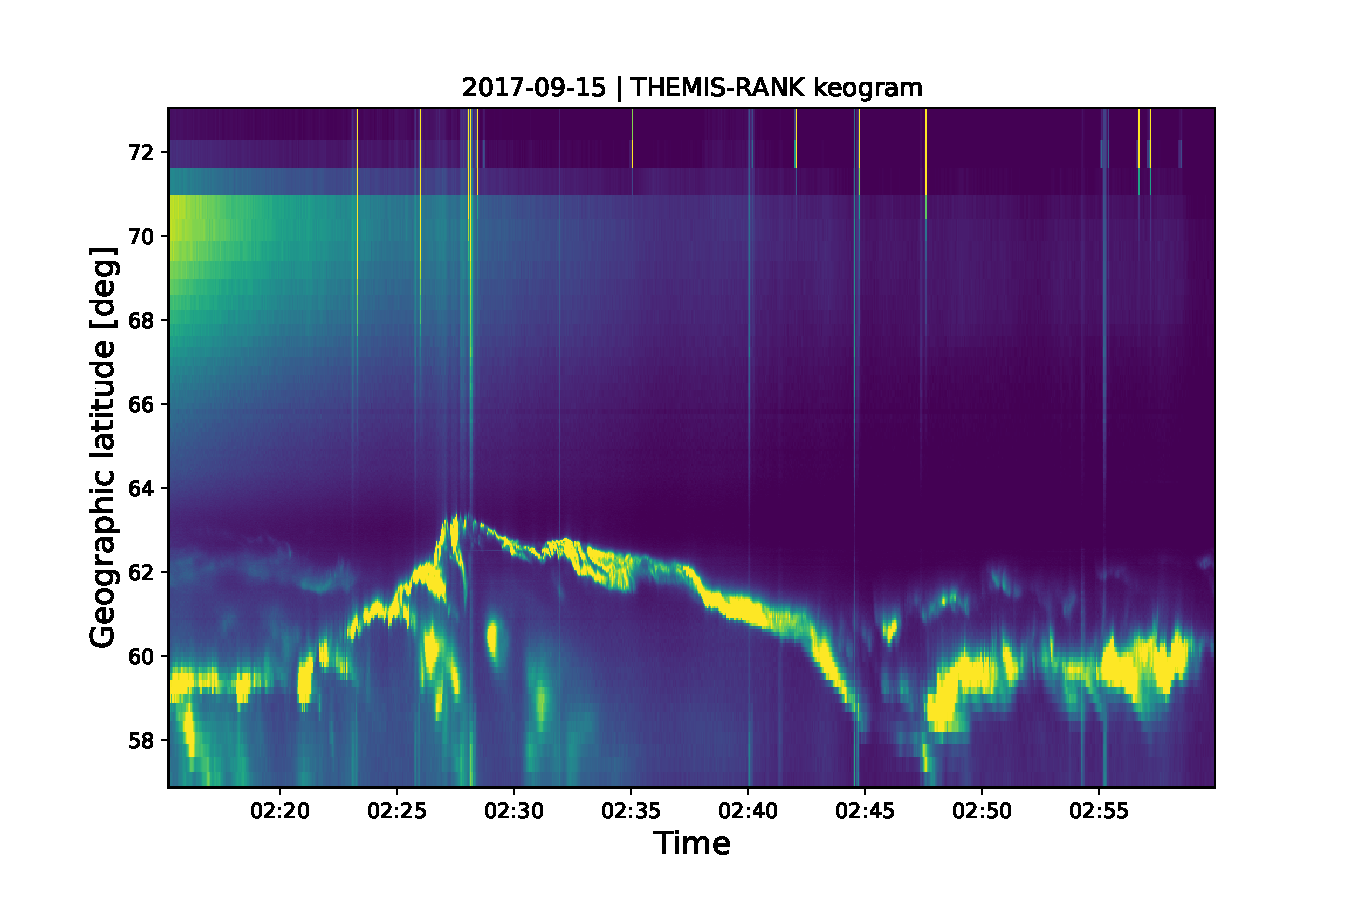
\includegraphics[width=\textwidth]{figures/fig3.png}
      \caption{A full-night keogram showing the dynamic aurora observed at Gillam, Canada. Panel a shows the unmapped keogram with the pixel index vertical axis, while panel b shows the latitude of the pixels mapped to 110 km altitude. \textcolor{red}{Add an AACGM keogram as well?}}
      \label{fig3}
\end{figure}


\subsection{Animating Images}
aurora-asi-lib allows the user to easily animate ASI fisheye images using \verb|asilib.animate_fisheye()|. It first saves png images in a unique subfolder in the \verb|asilib.config['ASI_DATA_DIR']/animations/images/| folder, and then animates them using the \verb|ffmpeg| \cite{ffmpeg} library. Animation S1 in the supporting information (SI) document shows an example of auroral streamers.

Animating just the fisheye images is somewhat limiting. Thus, \verb|asilib| also includes \verb|asilib.animate_fisheye_generator()| (which is technically a coroutine) to iterate over and pause after plotting each image---to enable you to modify each animation frame. Then, after the iteration is complete, \verb|asilib.animate_fisheye_generator()| combines the modified images into an animation. The user can make many different types of modifications, and we point the reader to the read the docs \textcolor{red}{add in link} to find the most recent list of modifications. As an example, you can use the  \verb|asilib.animate_fisheye_generator()| to superpose a satellite path and estimate the auroral intensity at its footprint during a conjunction. This is further described in the next two sections.

As the names imply, \verb|asilib.animate_map()| and \verb|asilib.animate_map_generator()| animate the projected images on a map. Both of these functions work in a similar manner to the \verb|animate_fisheye| functions. 

We mentioned earlier that the \verb|asilib.animate_fisheye_generator()| is technically a coroutine. So what does that mean? In this context, it means that before looping over each ASI image, you can request the images and time stamps from \verb|asilib.animate_fisheye_generator()| using the \verb|.send("data")| method. This approach appears rather contrived, however, a major advantage of this design is that the user sees exactly what ASI data the generator function will loop over. This is useful, for example, if you need the ASI time stamps to appropriately sample some other data such as a satellite's location. We will discuss one application of this in detail later.

\subsection{ASI analysis tools}
Currently, \verb|asilib| provides three functions that are useful for analyzing conjunctions: \verb|asilib.lla2footprint()|, \verb|asilib.lla2azel()|, and \verb|asilib.area2pixels()|.

\verb|asilib.lla2footprint()| uses IRBEM-Lib (\cite{irbem}; requires a separate installation and compilation of the Fortran source code) to trace a satellite's position, in geographic (latitude, longitude, altitude) (LLA) coordinates, along a magnetic field line. This field line is defined using one of the magnetic field models that are supported by IRBEM. The primary use of this function is to map a low Earth orbiting satellite's location at, for example, 500 km altitude, to its magnetic footprint at the assumed auroral emission altitude (e.g. 110 km for THEMIS or 230 km for REGO as previously mentioned).

The next function is \verb|asilib.lla2azel()|. This function maps the satellite's footprint location, in LLA coordinates, to the ASI's (azimuth, elevation) coordinates (AzEl) using the skymaps. This function returns both the AzEl coordinates as well as the corresponding pixel indices.

Lastly, \verb|asilib.area2pixels()| calculates a mask of pixels inside an auroral emission area. This function is useful to calculate the mean ASI intensity (or another statistical method) using pixels that map to a physical area in the sky. The mask contains 1s inside of the area and \verb|numpy.nan| outside of it. You then multiply the image with the mask: the pixel intensities outside of the area are then \verb|numpy.nan| and unchanged inside the area. We chose to use \verb|numpy.nan| to ensure that the mean of the intensity is correctly applied---it will fail if you call \verb|numpy.mean(image*mask)|, but \verb|numpy.nanmean(image*mask)| will ignore NaNs and correctly calculate the mean intensity inside the area)

By default, the area is 5x5 km. If the area is so small that not even one pixel is contained inside it (but it is above the horizon), \verb|asilib.area2pixels()| will slowly increase the area tolerance until at least one pixel is found. Lastly, if the area is completely outside of the skymap, \verb|asilib| will raise a warning and the corresponding mask will be all \verb|numpy.nan|. 

\subsection{An example: a satellite-ASI conjunction}\label{satellite_conjunction}
In this example we combine the aforementioned analysis functions to calculate the mean auroral intensity at the an imaginary satellite's footprint during a conjunction with a THEMIS ASI. The satellite orbits at a 500-km altitude low Earth orbit. We will calculate and the mean ASI intensity in a 20x20 km area at a 110 km altitude. And lastly, we will animate the conjunction.

For this example we use the satellite's location in LLA coordinates with time stamps that line up with the ASI times. In reality, the satellite and ASI time stamps are unlikely to line up, so you'll need to interpolate the satellite locations to the ASI time stamps.

Our analysis consists of three main steps. Step 1: we use \verb|asilib.lla2footprint()| to trace the satellite's position along the magnetic field line to 110 km. Step 2: we use \verb|asilib.lla2azel()| to find where in the imagers field of view (azimuth and elevation) the satellite's footprint was. Lastly, Step 3: we use \verb|asilib.area2pixels()| to identify the image pixels in the 20x20 km area around the footprint. We then use these pixels to calculate the mean ASI intensity as a function of time (and satellite position). These steps are implemented in the ``Figure 4" section of the \verb|asilib_figures| notebook.

Animation S2 shows the result of this conjunction analysis and Fig. \ref{fig4} shows a five-frame montage summarizing the animation. Fig. \ref{fig4}a-d show the fisheye lens images at the annotated time stamps. The complete satellite footprint path is represented by the red line and the instantaneous footprint by the red dot. The yellow areas around the footprints bound the 20x20 km area. Lastly, Fig. \ref{fig4}e shows the mean ASI intensity time series for the conjunction---it clearly shows the signature of the auroral arc between 2:33:30 and 2:34:15.

\begin{figure}
      \includegraphics[width=\textwidth]{figures/fig4.png}
      \caption{A conjunction montage of Animation S2. Panels a-d shows the auroral arc evolution and the satellite's location. The red line is the satellite track and the red dot is its instantaneous position. The yellow quadrilateral bounds the pixels inside the a 20x20 km area surrounding the satellite's 110 km altitude footprint. Lastly, panel e shows the mean ASI intensity, as a function of time, inside the yellow quadrilaterals. When the satellite passed through the arc between 2:33:30 and 2:34:15, the mean ASI show two corresponding intensity enhancements.}
      \label{fig4}
\end{figure}

\section{Quality Assurance}
We developed AuroraX with useability, reliability, and maintainability at the forefront. The source code for the the tools described here is open source and hosted on GitHub. It is also archived on Zenodo and the Python Packaging Index (PyPI). On GitHub you can submit an Issue for bugs or feature requests, and can contribute to AuroraX with a Pull Request.  

Documentation is critically important to the survival and usability of software and the AuroraX documentation is hosted at \url{https://docs.aurorax.space/}. There you will find installation instructions, examples, comprehensive tutorials, and a detailed API. The documentation source code is bundled with the software source code on GitHub, useful in case you need to recreate the documentation on a computer using the Sphinx Python document generator.

To ensure code stability, the aurora-asi-lib \textcolor{red}{and others?} source code comes with tests that you can run locally and that are automatically run on GitHub Actions every time a change is pushed to the repository. These comprehensive tests check and warn us of any software bugs that may arise during development.

Lastly, we use semantic versioning and a \verb|CAHNGELOG.md| to communicate all major, minor, and patch changes with the community. We made many backward-incompatible changes before version 1.0.0, but henceforth we will indicate future backward-incompatible changes with major releases (i.e. version X.0.0). 

\section{Conclusion}
The AuroraX website, PyAuroraX, and aurora-asi-lib tools provide the auroral science community with a simple and a robust set of analysis tools to enable more robust auroral system-level science. As we showed, AuroraX toolkit provides enables an end-to-end analysis solution. We described one such solution: to identify and analyze conjunctions. We showed how AuroraX website or PyAuroraX can be used to identify and filter conjunctions between an ASI and a satellite. Auroral researchers can then use aurora-asi-lib to carefully analyze this and other data. This example is just one way that AuroraX can help you quickly sift through an immense volume of ASI data to uncover new physics.

In the near future we will add more ASI arrays and satellites to AuroraX. TREx and other ASIs will be added to aurora-asi-lib through future work from the current development team and the help of community developers. However, standardizing the ASI data format is crucial to this endeavor and will enable future quick addition of new ASI data to this code infrastructure. Additionally, the continued success and usability of AuroraX is dependent on the community contributing to the development of this tool. We encourage an open science approach and look forward to working more broadly within the Auroral research community.  \textcolor{red}{I am unsure what else to add here. Ideas?}

\section*{Conflict of Interest Statement}
The authors declare that the research was conducted in the absence of any commercial or financial relationships that could be construed as a potential conflict of interest.

\section*{Author Contributions}
DC developed the AuroraX website and pyaurorax. AJH, KRM, and IT assisted MS with developing aurora-asi-lib. MS, BGL, and DC wrote the manuscript. ED, ELS, and DC provided the THEMIS and REGO ASI data and expertise.  All authors contributed to manuscript revision, read, and approved the submitted version.

\section*{Funding}
MS and BGL acknowledge the support provided by the NASA Postdoctoral Program at the NASA's Goddard Space Flight Center, administered by Oak Ridge Associated Universities under contract with NASA. AJH was supported in part by the Goddard Internal Funding Model which funds the Space Precipitation Impacts team with grant HISFM21. \textcolor{red}{What about Calgary's funding sources?}

\section*{Acknowledgments}
We are thankful for the engineers and scientists who made the AuroraX, THEMIS ASI, and REGO ASI projects possible. M. Shumko and B. Gallardo-Lacourt acknowledge the support provided by the NASA Postdoctoral Program at the NASA’s Goddard Space Flight Center, administered by Oak Ridge Associated Universities under contract with NASA. A. Halford and K.R. Murphy were supported by the GSFC's Space Precipitation Impacts (SPI) Internal Scientist Funding Model. \textcolor{red}{Other acknowledgments.}

\section*{Data Availability Statement}
The datasets and code presented here can be found in the following links.
\begin{itemize}
    \item AuroraX: \url{https://aurorax.space/} and \url{https://github.com/aurorax-space}
    \item AuroraX documentation: \url{https://docs.aurorax.space}
    \item aurora-asi-lib: \url{https://aurora-asi-lib.readthedocs.io/en/latest/}
    \item THEMIS: \url{https://data.phys.ucalgary.ca/sort_by_project/THEMIS/asi/}
    \item REGO: \url{https://data.phys.ucalgary.ca/sort_by_project/GO-Canada/REGO/}
\end{itemize}

\section*{Contribution to the Field Statement}
\noindent The aurora is a ubiquitous light spectacle that has been observed in the polar regions for millennia. The regional scale of the aurora has led to the recent development of numerous imagers---and arrays of imagers---that continuously take images thorough the night. The image volume has quickly become unmanageable by any single group of scientists, so the imager datasets are at best fragmented on the internet, and at worst hidden from the public. The AuroraX project aims to address this problem by combining the publicly-available datasets into one easily accessible location. This project consists of three main tools:  the AuroraX website (\url{https://aurorax.space/}); PyAuroraX, a application program interface to the AuroraX website written in Python; and aurora-asi-lib, an auroral all-sky imager library also written in Python. Together, these three tools make the auroral data easily accessible to the public and the scientific community---so that we can all enjoy the dancing lights.

\bibliographystyle{Frontiers-Harvard} 
\bibliography{refs}
\end{document}